\subsection{Methods}
In this section the different methods used to solve the Learning from Demonstration approaches are presented. The paragraphs are organized according to the temporal order in which the different approaches were proposed for the context of interest. So the first paragraph will be devoted to methods related to Behavioral Cloning. A brief presentation will be made on methods related to Inverse Reinforcement Learning. In conclusion, recent methods related to Generative Adversarial Imitation Learning and Learning from Observation will be described and analyzed.
\label{sec:methods}
\paragraph{Behavioral Cloning (BC). [MAX 5]} \mbox{} \\ 
Behavioral Cloning is one of the first approaches used to learn a task from a set of demonstrations. It is framed as a Supervised Learning problem, solved through Algorithm \ref{alg:bc}. In this setting there are at least to questions to answer: 
\begin{enumerate*}[label=\textbf{(\arabic*)}]
    \item Choose whether to optimize in trajectory space or action space.  
    \item What kind of representation to use for the policy.
\end{enumerate*}
Generally speaking, Algorithm \ref{alg:bc} defines the procedure used to solve the learning task, given the dataset $\mathcal{D}^{E}$, a parameterized learner policy $\pi^{L}_{\theta}$, and a loss-function $\mathcal{L}$, the goal is to find the policy parameter that minimizes the loss-function, in other terms, $\theta^{*} = \underset{\theta}{argmin} \ \mathbb{E}_{(\boldsymbol{\tau}, \mathbf{c}) \sim \mathcal{D}^{E}} \ [\mathcal{L}((\boldsymbol{\tau}, \mathbf{c}), \ \pi^{L}_{\theta})]$.
\newline According to \cite{osa2018algorithmic,zheng2021imitation_progress_taxonomies_opportunities}, BC methods can be categorized as Model-Free and Model-Based, and based on the fact that the policy is optimized either in the trajectory space or in the action space.
\begin{algorithm}
\caption{Abstract Algorithm for Behavioral Cloning}\label{alg:bc}
\begin{algorithmic}
\Require A set of expert demonstrations $\mathcal{D}^{E}$, a parameterized policy $\pi_{\theta}^{L}$
\Ensure The optimal set of policy parameter $\theta^{*}$
\State Optimize $\mathcal{L}$ w.r.t. policy parameter $\theta$ using $\mathcal{D}^{E}$
\end{algorithmic}
\end{algorithm} 

\textbf{Model-Free methods} learns a policy that reproduces the expert's behavior without learning/estimating system dynamics. Since they do not require neither to estimate the system dynamic nor to learn a reward function, they are simple to implement and do not necessary require system  interactions. 

Model-Free methods that derive policy in the space of trajectories were very popular in the context of Model-Free BC for robotic manipulation trajectory planning, given their ability to explicitly model constraints on the generated trajectory (e.g. a smooth convergence to the goal state). Indeed, in this setting very popular and studied methods are the \textit{Dynamic Movement Primitives} (DMPs) \cite{ijspeert2002learning,ijspeert2013dynamical}, and the \textit{Probabilistic Movement Primitives} (ProMPs) \cite{}. \textcolor{red}{[To continue...]}

Regarding the methods that derive the policy in the action-space. One of the primal work is such setting was \cite{pomerleau1988alvinn}, which proposed \textit{ALVINN}, an autonomous vehicle driving system based on a Neural Network, that infers the steering angle, given a camera image as input. The network was trained on pairs (image, steering-angle), the steering-angle was discretized over 45 units, and the training was defined as a supervised classification problem. This work immediately emphasized the problem of compounding-error, caused by covariate-shift phenomena. This issue occurs because an action $a_{t}$ influences the next state $s_{t+1}$, violating the i.i.d assumption of Supervised Learning, and generating a test-data distribution, that may be different from the the training one. This phenomena has a relevant consequence on the expected performance of the system. Indeed, assuming to have a system that makes an error with probability $\epsilon$, and a task with time-horizon $T$, then, due to compounding error, a supervised learner reaches a total cost of $O(\epsilon \ T^{2})$, rather than $O(\epsilon \ T)$ \cite{ross2010efficient_reductions,ross2011dagger}. To attenuate this problem, interactive supervised learning algorithms have been proposed, such as the well-known \textit{DAgger} \cite{ross2011dagger}. Algorithm \ref{alg:dagger} describes the DAgger procedure. It is an aggregation strategy, based on the idea to train the policy $\pi$ under the state-distribution induced by the policy itself, but with the correct action performed by the expert. the main problem with DAgger is that it requires the expert to interact with the system during the training, introducing both safety and data-efficiency problems, especially when the system does not provide the human expert with sufficient control authority during the sampling process \cite{laskey2017comparing_hc_rc}. \begin{algorithm}
\caption{DAgger Algorithm \cite{ross2011dagger}}\label{alg:dagger}
\begin{algorithmic}
\Require Initial Dataset $D \leftarrow \emptyset$, Initial policy $\pi^{L}_{1}$
\Ensure The best policy $\pi^{L}_{i}$
\For {$i=1, \dots N$}
    \State Sample $T-step$ trajectories using $\pi^{L}_{i}$
    \State Let $D_{i} = {(s_{t}, \pi^{E}(s_{t}))}$, state $s_{t}$ visited by policy $\pi^{L}_{i}$, 
    \State and actions given by the expert
    \State Aggregate Dataset, $D \leftarrow D \bigcup D_{i}$
    \State Train policy $\pi^{L}_{i}$ on $D$
    \State Let $\pi^{L}_{i+1} = \beta_{i}\pi^{E} + (1- \beta_{i})\pi^{L}_{i}$
\EndFor
\end{algorithmic}
\end{algorithm}
\newline Human-Guided DAgger (HG-DAgger) \cite{kelly2019hg_dagger} is an extension of the classic DAgger strategy, in which the human expert observes the rollout of the current policy, so if the agent has entered an unsafe region of the state space, the expert takes control and guides the system to a safe and stable region. In \cite{jang2022bc_z} was shown how HG-DAgger can be effectively used in the context of robotic manipulation. Indeed, starting from the same total number of episodes, a policy trained with only expert demonstration has a significantly lower success rate than a policy trained on a dataset with both expert demonstration and expert adjustments. In the context of Interactive Learning for Robot Manipulation, other works of interest include \cite{mandlekar2020human_in_the_loop,chisari2022correct}. In \cite{chisari2022correct}, a human expert provides both corrective and evaluative feedback. %(Figure \ref{fig:feedback}).
The former consists in the human that takes control of the robot to adjust the trajectory, the latter consists in a scalar weight $q$, set to 1 if the trajectory is satisfactory, 0 the trajectory is not satisfactory, $\alpha$ if the trajectory is adjusted by the expert, where $\alpha$ is the ration between non-corrected and corrected samples. Then a Neural Network % in Figure \ref{fig:architecture}
was trained by minimizing a weighted version of the maximum-likelihood $\mathcal{L}(a_{t},s_{t}) = - q \ log(\pi^{L}_{\theta}(a_{t}|s_{t}))$. Real-world experiments show that with a training time of \textbf{41 minutes}, including environmental reset, it is possible to have an agent capable of performing tasks such as picking up a cube or pulling a plug.
%\begin{figure}[htbp]
    \begin{subfigure}{0.45\textwidth}
         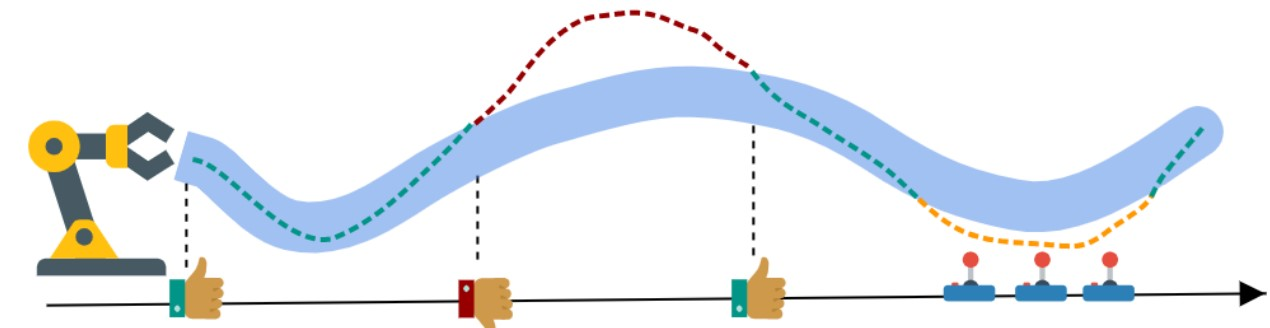
\includegraphics[width=\textwidth]{Figures/images/correct-me-if-i-am-wrong/feedback.jpg}
         \caption{Evaluative feedback: the expert labels the sub-trajectory as satisfactory or not. Corrective feedback: the human guides the robot towards the correct trajectory}
         \label{fig:feedback}
    \end{subfigure}
    \hfill
    \begin{subfigure}{0.50\textwidth}
         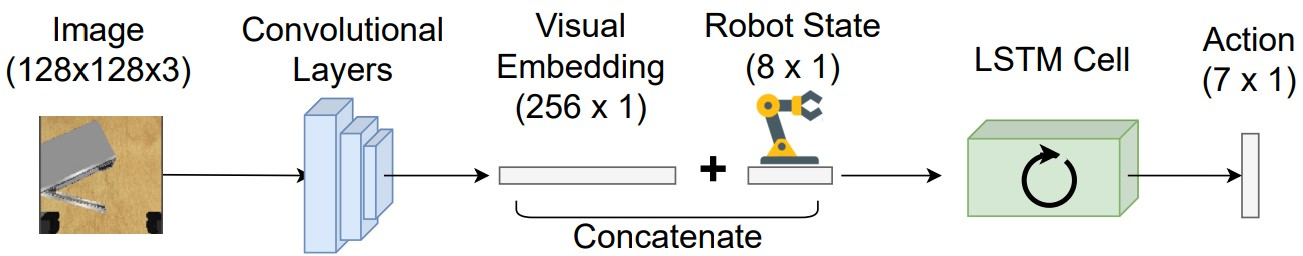
\includegraphics[width=\textwidth]{Figures/images/correct-me-if-i-am-wrong/correct_me_architecture.jpg}
         \caption{Policy architecture: The input is an RGB image of the scene, the output is the desired end-effector pose and the gripper state}
         \vspace{0.5cm}
         \label{fig:architecture}
    \end{subfigure}
    \caption{(\ref{fig:feedback}) Representation of the meaning of the feedback, (\ref{fig:architecture}) Policy architecture proposed in \cite{chisari2022correct}}
    \label{fig:correct_me_if_im_wrong}
\end{figure}

%Classic Behavioral Cloning

Despite the covariate-shift problem, \cite{zhang2018deep_vr_teleoperation} showed that very interesting performance can be obtained in the context of Robot Manipulation Task, by means of Behavioral Cloning and high quality demonstrations given by teleportation system. In this work, a CNN was trained to predict the desired linear-velocity and angular-velocity of the end-effector, with the binary gripper state (open/close), given in input the current RGB-D observation of the scene, and the position of three points of the end-effector, during the last 5 time-steps. The system was tested on 10 tasks, and the performance are reported in Table \ref{table:deep_vr_teleoperation_results}.
\begin{table}
\centering
\caption{Statistics of Training set, and Test Success rate \cite{zhang2018deep_vr_teleoperation}}
\label{table:deep_vr_teleoperation_results}
\resizebox{\linewidth}{!}{%
\begin{tabular}{c|c|c|c|c|c|c|c|c|c|c}
task                                                                                                                                   & reaching & grasping & pushing & plane & cube & nail & grasp-and-place & grasp-drop-push & grasp-place-x2 & cloth  \\ 
\hline
\rowcolor[rgb]{0.753,0.753,0.753} \#demo                                                                                               & 200      & 180      & 175     & 319   & 206  & 215  & 109             & 100             & 60             & 100    \\ 
\hline
\begin{tabular}[c]{@{}c@{}}demo duration \\(min)\end{tabular}                                                                          & 13.7     & 11.1     & 16.9    & 25.0  & 12.7 & 13.6 & 12.3            & 14.5            & 11.6           & 10.1   \\ 
\hline
\rowcolor[rgb]{0.753,0.753,0.753} \begin{tabular}[c]{@{}>{\cellcolor[rgb]{0.753,0.753,0.753}}c@{}}Test success rate\\(\%)\end{tabular} & 91.6     & 97.2     & 98.9    & 87.5  & 85.7 & 87.5 & 96.0            & 83.3            & 80.0           & 97.4  
\end{tabular}
}
\end{table}
% Meta-Learning, few shot, zero-shot. Il problema principale è che per l'esecuzione di differenti task c'è bisogno di riaddestrare da zero le policy
\newline One important aspect to note is that for each task the network was trained from scratch. This is not a desired property for a highly adaptable system, as stated in Section \ref{sec:intro}. For this reason, methods based on Meta-Learning algorithms have been proposed. The idea behind Meta-Learning is to train a model on a variety of tasks, in such a way that it can solve a new tasks, using only a small number of training samples \cite{finn2017maml}. Algorithm \ref{alg:maml} describes the steps followed by the \textit{Model-Agnostic Meta-Learning} (MAML) algorithm \cite{finn2017maml}, that is the base for different methods which apply One-shot Imitation Learning in the context of Behavioral Cloning \cite{finn2017one_shot_visual_il,yu2018daml,yu2018one_shot_hil}.\begin{algorithm}[h]
\caption{Model-Agnostic Meta-Learning (MAML) \cite{finn2017maml}}
\label{alg:maml}
\begin{algorithmic}
\Require Distribution over tasks $p(\mathcal{T})$
\State Randomly initialize $\theta$
\While {$i=1, \dots N$}
    \State Sample batch of tasks $ \mathcal{T}_{i} \sim p(\mathcal{T})$
    \For {\textbf{all} $\mathcal{T}_{i}$}
        \State Evaluate $\nabla_\theta \mathcal{L}_{\mathcal{T}_{i}}(f_{\theta})$ w.r.t. $K$ examples
        \State Compute adapted parameters with gradient descent: $\theta'_{i} = \theta - \alpha \nabla_\theta\mathcal{L}_{\mathcal{T}_{i}}(f_{\theta})$
    \EndFor
    \State Update $\theta \leftarrow \theta - \beta \nabla_\theta \sum_{\mathcal{T}_{i} \sim p(\mathcal{T})} \mathcal{L}_{\mathcal{T}_{i}}(f_{\theta'_{i}})$
\EndWhile
\end{algorithmic}
\end{algorithm}
\newline In \cite{finn2017one_shot_visual_il}, MAML algorithm was used to prove the effectiveness of Meta-Learning in the context of real robot manipulation, with visual observations, as opposite to \cite{duan2017one_shot_il}. A CNN was trained by following the Algorithm \ref{alg:maml}, using as loss-function the Mean Squared Error, computed between the predicted action and the ground truth one. For real-robot experiments a dataset of 1300 placing demonstrations (i.e. place an holded object in a target container), containing near to 100 different objects, was collected through teleportation. The trained system was tested by performing the adaptation step on one video demonstration, over 29 new objects, moreover, between the video demonstration and the actual execution, the objects configuration was changed. In this setting the system reached the $\mathbf{90\%}$ of success rate, outperforming baseline methods based on LSTM \cite{duan2017one_shot_il}, and contextual network (i.e. a CNN that takes in input the current observation and the image representing the target state).
\newline In \cite{yu2018daml}, the \textit{Domain Adaptive Meta-Learning} algorithm (DAML) was proposed with the goal of learning to infer a policy from a single human demonstration. To achieve it, a two-step algorithm was proposed. In the first-step, called \textbf{Meta-Learning step}, given in input, for each task $\mathcal{T}$, a set of human demo $\mathcal{D}^{h}_{\mathcal{T}}$ and a set or robot demo $\mathcal{D}^{r}_{\mathcal{T}}$ (Figure \ref{fig:daml}), the \textit{initial policy parameters} $\theta$ and the \textit{adaptive loss} parameters $\psi$ are learned, solving the problem in Formula \ref{eq:daml}. \begin{equation}
 \label{eq:daml}
 \underset{\theta,\psi}{\min} \sum_{\mathcal{T} \sim p(\mathcal{T})} \sum_{\mathbf{d}^{h} \sim D^{h}_{\mathcal{T}}} \sum_{\mathbf{d}{^r} \sim D^{r}_{\mathcal{T}}} \mathcal{L}_{BC}(\theta - \alpha \nabla_\theta\mathcal{L}_{\psi}(\theta,\mathbf{d}^{h}), \mathbf{d}^{r})
\end{equation}

\newline Where the outer loss is $\mathcal{L}_{BC}(\phi,\mathbf{d^{r}}) = \sum_{t} log(\pi_{\phi}(a_{t}|s_{t},o_{t}))$, and the inner-loss $\mathcal{L}_{\psi}$, is the learned adaptive loss, which is used during the \textbf{Meta-Test step}, where the policy parameters are adapted with gradient descent given in input a video of human demo of a new task $\mathcal{T}$, i.e. $\psi_{\mathcal{T}} = \theta - \alpha \nabla_{\theta} \mathcal{L}_{\psi}(\theta, \mathbf{d^{r}})$. Experimental evaluation on tasks such as placing, pushing, and pick-and-place, has shown that: \begin{enumerate*}[label=\textbf{(\alph*)}]
    \item The system was able to generalize across both new objects and objects configuration starting from only a single human-demonstration.
    \item A performance degradation was observed in large domain-shift experiments, such as novel backgrounds and different camera view-points.
\end{enumerate*}
The work proposed in \cite{yu2018one_shot_hil} is an extension of DAML, for multi-stage tasks, i.e. tasks that are composed of different motion primitives. \begin{figure}[htbp]
    \centering
    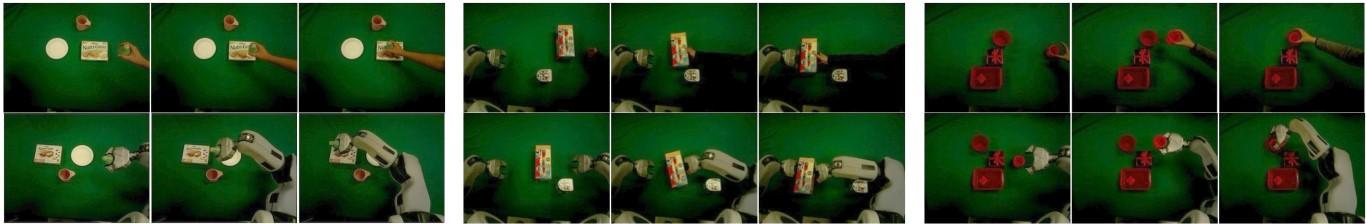
\includegraphics[width=\textwidth]{Figures/images/daml/tasks.jpg}
    \caption{Tasks performed in \cite{yu2018daml}. (Top row) Human demonstration, (Bottom row) robot demonstration. (Left) Placing task, (Middle) pushing task, (Right) pick-and-place task.}
    \label{fig:daml}
\end{figure}


Generally speaking, all the works described up to now, consider the task distribution $p(\mathcal{T})$ as composed of one-single task, but with many different variations \cite{finn2017one_shot_visual_il} or different, but related tasks \cite{yu2018daml}. Very recent methods try to generalize BC to a huge variety of tasks \cite{jang2022bc_z,mandi2022towards_more_generalizable_one_shot}, 
In \cite{jang2022bc_z}, a large-scale dataset containing \textbf{100} diverse manipulation tasks was collected. The demonstrations were collected through expert teleoperation and shared autonomy process (DAgger \cite{ross2011dagger}). The demonstrated tasks were related to pick-and-place, grasp, pick-and-drag, pick-and-wipe, and push skills. The dataset was used to train the network in Figure \ref{fig:bcz_architecture}. As it can be noted the samples were composed by current robot observation, and a conditioning represented by either a vocal command or a video demo. The idea was that training a conditioned policy over the current observation $o_{t}$, and a task representation $c_{t}$, $\pi^{L}(a_{t}|o_{t}, c_{t})$, it would allow the policy to generalize over new tasks in a zero-shot manner (i.e. without any fine-tuining). Experimental results shown that, over 28 held-out tasks, containing both completely new object, and known objects but in different tasks, an average success rate of \textbf{38\%} was reached in the easiest setting, with only one distractor and with language conditioning. The success rate dropped to \textbf{4\%} in the hardest setting with 4 distractors and video conditioning. These bad performance can be justified by the classic training procedure followed, while different advantages may be gained from Meta-Learning algorithms, and the way in which the human video embedding was obtained, through a CNN on a 4x5 matrix
of images, with a completely loss of temporal information.
\begin{figure}[htb!]
    \centering
    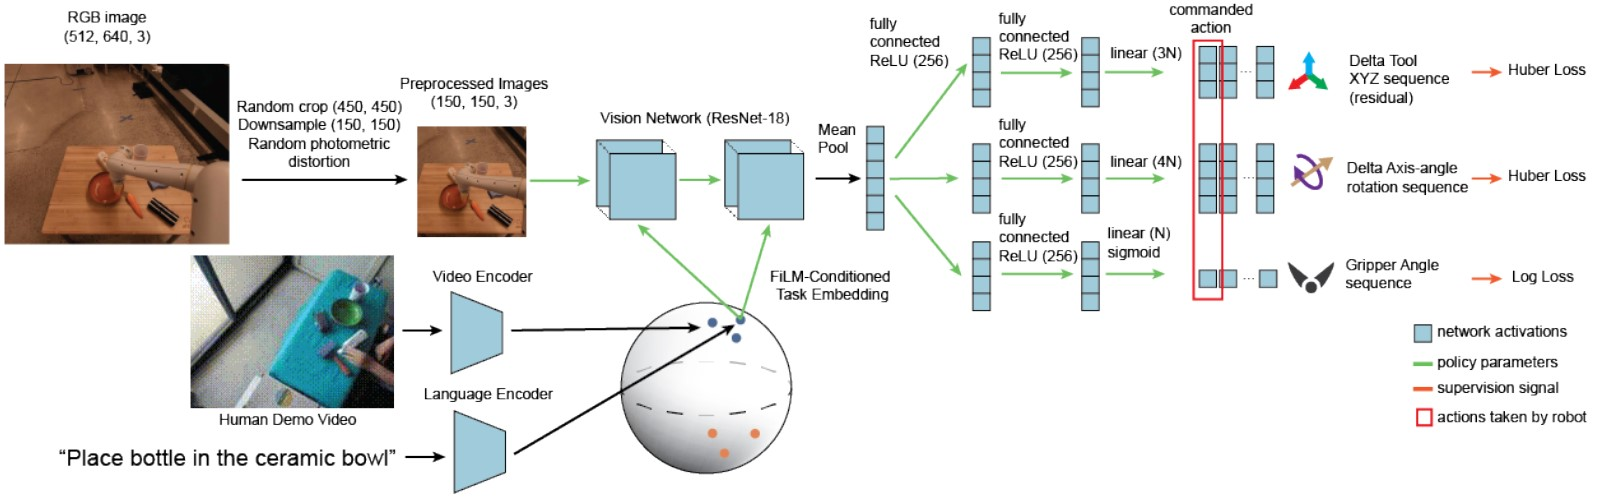
\includegraphics[width=0.9\textwidth]{Figures/images/bc_z/bc-z-network.jpg}
    \caption{Architecture proposed in \cite{jang2022bc_z}}
    \label{fig:bcz_architecture}
\end{figure}


\textbf{Model-Based methods},


\paragraph{Inverse Reinforcement Learning (IRL) [MAX 2]}  \mbox{} \\
Inverse Reinforcement Learning or Inverse Optimal Control is a Learning from Demonstration approach that was introduced in \cite{abbeel2004apprenticeship}. In IRL, starting from a set of expert-demonstrated trajectories, the main goal is to obtain the \textit{Reward function} $R$, which explains the expert behavior. Once $R$ is found, an RL algorithm is run to obtain the policy $\pi^{L}_{\theta}$ (Algorithm \ref{alg:irl}). \begin{algorithm}
\caption{Classic feature matching IRL algorithm}
\label{alg:irl}
\begin{algorithmic}
\label{alg:irl_algorithm}
\Require Dataset of expert trajectories $D = \left \{ \boldsymbol{\tau}^{E}_{i} \right \}^{N}_{i=1}$ 
\Require Reward function $R_{\omega}$, policy $\pi^{L}_{\theta}$ 
\While {policy improves}
    \State Evaluate the state-action visitation frequency $\mu$ of the current policy $\pi^{L}_{\theta}$
    \State Evaluate the objective function $\mathcal{L}$, w.r.t. $\mu$ and the dataset $D$
    \State Update the reward-function parameters $\omega$ based on $\mathcal{L}$
    \State Update the policy $\pi^{L}_{\theta}$ through a RL algorithm, using the updated $r_{\omega}$
\EndWhile
\end{algorithmic}
\end{algorithm}%Algorithm \ref{alg:irl_algorithm} summarizes the classic procedure followed by a IRL method. It is an iterative procedure characterized by two set of parameters, $\omega$ for the reward function, and $\theta$ for the policy $\pi^{L}_{\theta}$. 
An important design choice is related to how parametrize the reward-function, i.e. a \textbf{linear} function of the features \cite{ratliff2006maximum_margin,ziebart2008maximum_entropy} or  a \textbf{non-linear} function of the features \cite{ratliff2009learning_to_search,wulfmeier2015deep_inverse_rl,finn2016guided_cost_learning}.
Generally, the IRL algorithms are characterized by the following problems: \begin{enumerate*}[label=\textbf{(\arabic*)}]
    \item The learning process could be time-consuming and impractical for high-dimensional problems, because of the double-nested optimization procedure.  
    \item The IRL problem is \textit{ill-posed}, since there are different reward-functions that could lead to the same action.
\end{enumerate*}
%\begin{algorithm}
\caption{Classic feature matching IRL algorithm}
\label{alg:irl}
\begin{algorithmic}
\label{alg:irl_algorithm}
\Require Dataset of expert trajectories $D = \left \{ \boldsymbol{\tau}^{E}_{i} \right \}^{N}_{i=1}$ 
\Require Reward function $R_{\omega}$, policy $\pi^{L}_{\theta}$ 
\While {policy improves}
    \State Evaluate the state-action visitation frequency $\mu$ of the current policy $\pi^{L}_{\theta}$
    \State Evaluate the objective function $\mathcal{L}$, w.r.t. $\mu$ and the dataset $D$
    \State Update the reward-function parameters $\omega$ based on $\mathcal{L}$
    \State Update the policy $\pi^{L}_{\theta}$ through a RL algorithm, using the updated $r_{\omega}$
\EndWhile
\end{algorithmic}
\end{algorithm}
\newline To solve the problem of multiple solutions some constraints to the optimization procedure have to be added, based on the constraint type, the two main IRL procedures can be identified: \begin{enumerate*}[label=\textbf{(\alph*)}]
    \item The \textit{Maximum Margin Prediction} (MMP) approach \cite{ratliff2006maximum_margin,ratliff2009learning_to_search}.  
    \item \textit{Maximum Entropy} (Max-Ent) approach \cite{ziebart2008maximum_entropy,wulfmeier2015deep_inverse_rl,finn2016guided_cost_learning}.
\end{enumerate*}
The MMP methods assume that the demonstrated trajectories are optimal and work in a deterministic setting. The aim is to find the cost-function where the reward of the demonstrated trajectories $R(\boldsymbol{\tau}^{E})$ is greater than the reward of all the alternative trajectories $R_{\omega}(\boldsymbol{\tau})$, by a certain margin $m$, i.e. $ \underset{\omega, m}{\max} \ m \  \ s.t. \ R_{\omega}(\boldsymbol{\tau}^{E}) \geq \max (R_{\omega}(\boldsymbol{\tau})) + m$. The main problem with this formulation is that it does not handle the case in which the expert behavior is sub-optimal, leading to an ambiguous notion of margin. To handle this problem the Max-Ent approach has been proposed in \cite{ziebart2008maximum_entropy}. In Max-Ent the goal is to find the reward-function parameters $\psi$ that drives the policy to maximize the entropy, subject to the feature expectation matching, i.e $\underset{\psi}{\max} \ \mathcal{H}(\pi^{r_{\psi}}) \ s.t. \ \ \mathbb{E}_{\pi^{r_{\psi}}}[\mathbf{f}] = \mathbb{E}_{\pi^{*}}[\mathbf{f}]$. The setting based on the Maximum Entropy is the most popular setting in the IRL field since it removes the ambiguous aspects of the previous formulation. In the original work, the reward-function was a linear combination of the features, i.e. $r_{\psi} = \psi^T \mathbf{f}$. This reward formulation is not suited for high-dimensional feature space, which can require the capability to model non-linear reward structures. In \cite{wulfmeier2015deep_inverse_rl}, a deep-network was used to model the reward-function. In this work, the NN maps the feature vector $\textbf{f}$ into the reward value, and trained according to the Maximum-Entropy setting. Experimental results have shown that the NN ability to approximate highly nonlinear reward functions is essentially to successfully solve tasks in high-dimensional discrete state spaces. A generalization to continuous state-space was proposed in \cite{finn2016guided_cost_learning}. In particular, \cite{finn2016guided_cost_learning} faced the problem of learning a cost function in a high-dimensional continuous state space, with \textbf{unknown dynamics}. Indeed, starting from the exponential trajectory distribution $p(\tau) = \frac{1}{Z} \ exp(-c_{\theta}(\tau))$, the main difficulty is the estimation of the partition function $Z$, needed to compute the negative log-likelihood loss function $\mathcal{L}(\theta) = \frac{1}{N} \underset{\tau^{E}_{i} \in D_{demo}}{\sum} c_{\theta}(\tau^{E}_{i}) + \log(Z)$. Since, the dynamic is unknown the idea was to estimate the partition function through the trajectories obtained from the current policy rollouts, with the idea that during the learning of the cost function the current policy drives the distribution towards regions where samples are more useful.%i.e. $\mathcal{L}(\theta) \approx  \frac{1}{N} \underset{\tau^{E}_{i} \in D_{demo}}{\sum} c_{\theta}(\tau^{E}_{i}) +  \log \frac{1}{M} \underset{\tau^{L}_{j} \in D_{samp}}{\sum} \frac{exp(-c_{\theta}(\tau^{L}_{j}))}{q(\tau_{j})}$.
\begin{algorithm}[htbp]
\caption{Guided-Cost-Learning Algorithm \cite{finn2016guided_cost_learning}}
\label{alg:guided_cost_learning}
\begin{algorithmic}
\Require Initial controller $q_{k}(\tau)$ 
\For {i = 1, \dots, N}
    \State Generate $D_{traj}$ from $q_{k}(\tau)$
    \State $\mathcal{D}_{samp} \leftarrow \mathcal{D}_{samp} \bigcup \mathcal{D}_{traj}$
    \State Update the cost-function parameters, using $\mathcal{D}_{samp}$ and $\nabla_{\theta}\mathcal{L(\theta)}$
    \State Update the controller $q_{k+1}(\tau) \leftarrow q_{k}(\tau)$ according to \cite{levine2014lqr_flm} and using $\mathcal{D}_{traj}$
\EndFor
\end{algorithmic}
\end{algorithm}\label{lqr} Starting from these considerations, the Algorithm \ref{alg:guided_cost_learning} was proposed. The controller was obtained as a result of a Linear-Quadratic Regulator (LQR) optimization procedure, which returns a \textit{linear-gaussian policy}, $\pi(a_{t}|s_{t}) = \mathcal{N}(K_{t}s_{t} + k_{t}, S_{t})$, which optimizes a \textit{quadratic-cost function}, $c(s_{t},a_{t}) = \begin{bmatrix} s_{t} \\ a_{t} \end{bmatrix}^{T}C_{t}\begin{bmatrix} s_{t} \\ a_{t} \end{bmatrix} + \begin{bmatrix} s_{t}\\a_{t}\end{bmatrix}^{T} c_{t} + cc_{t}$,under the assumption of \textit{linear-gaussian dynamics} $s_{t+1} \sim P(s_{t+1}|s_{t},a_{t}) = \mathcal{N}(F_{t}\begin{bmatrix}s_{t}\\ a_{t}\end{bmatrix} + f_{t}, \Sigma_{t})$. The cost-function was parameterized according to a Neural Network, and experiments performed on real-robot manipulation tasks such as dish placement and pouring proved the effectiveness of the proposed method, outperforming the classic Max-Ent method.
%\begin{equation}
\label{formula:linear_gaussian_controller}
    \pi(a_{t}|s_{t}) = \mathcal{N}(K_{t}s_{t} + k_{t}, S_{t})
\end{equation}

\begin{equation}
\label{formula:quadratic_cost_function}
c(s_{t},a_{t}) = \begin{bmatrix}
s_{t}
\\ 
a_{t}
\end{bmatrix}^{T}C_{t}\begin{bmatrix}
s_{t}
\\ 
a_{t}
\end{bmatrix} + \begin{bmatrix}
s_{t}
\\ 
a_{t}
\end{bmatrix}^{T} c_{t} + cc_{t}
\end{equation}

\begin{equation}
\label{formula:gaussian_dyn}
s_{t+1} \sim P(s_{t+1}|s_{t},a_{t}) = \mathcal{N}(F_{t}
\begin{bmatrix}
s_{t}
\\ 
a_{t}
\end{bmatrix} + f_{t}, \Sigma_{t})
\end{equation}



\newline Recent method \cite{das2021model_based_irl_from_vd} tried to move IRL towards more complex learning scenario, such as learning a reward function from video-demonstrations. In \cite{das2021model_based_irl_from_vd} the architecture in Figure \ref{fig:model_based_irl} was proposed. The goal was to obtain the parameters of a cost function $C_{\Psi}(\hat{\boldsymbol{\tau}}, z_{goal})$, such that it was possible to derive a sequence of actions by minimizing the cost-function itself, $\textbf{a}_{new} \ = \ \textbf{a} \ - \ \eta \nabla_{a} C_{\Psi}(\hat{\boldsymbol{\tau}}, z_{goal})$, Different cost functions have been proposed, but all with the same objective to reduce the distance between the current predicted keypoints and the goal keypoints configuration. The trajectory $\hat{\boldsymbol{\tau}}$ is a a sequence of predicted states $[\hat{s}_{1}, \dots, \hat{s}_{T}]$, result of a learned dynamic model, $\hat{s}_{t+1} = f_{dyn}(\hat{s}_{t}, a_{t})$. Experimental results have shown that it is possible to learn a cost-function starting from human/robot video demonstrations. However, the proposed setting was tested on a very simple reaching task, proving how a lot of work has to be made in order to prove the effectiveness or ineffectiveness of IRL in complex real-robot manipulation tasks, starting from video demonstrations.
\begin{figure}[htb]
    \centering
    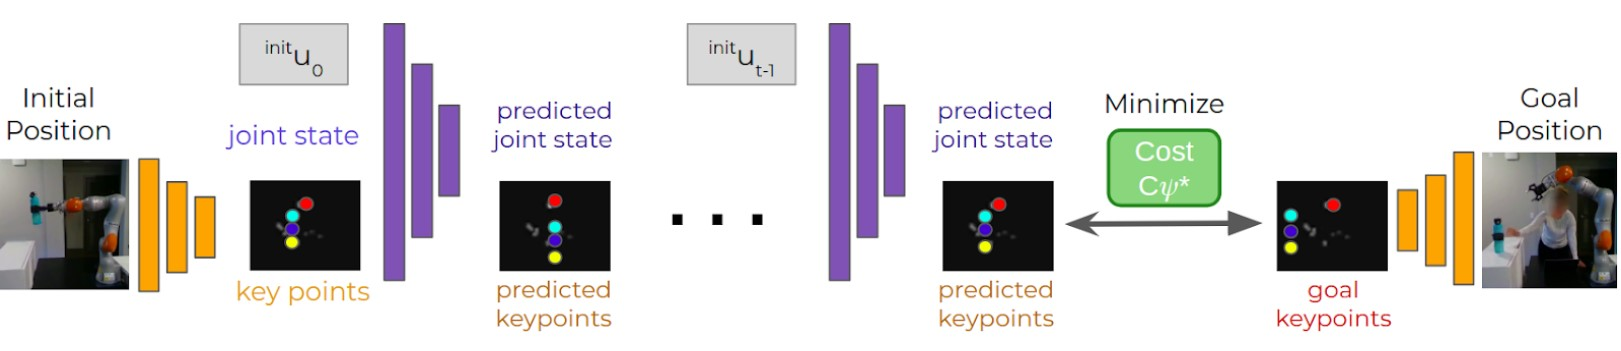
\includegraphics[width=\textwidth]{Figures/images/model_based_irl/model_based_irl.jpg}
    \caption{Architecture proposed in \cite{das2021model_based_irl_from_vd}}
    \label{fig:model_based_irl}
\end{figure}

\paragraph{Generative Adversarial Imitation Learning (GAIL) [MAX 5]} \mbox{} \\
Generative Adversarial Imitation Learning was proposed for the first time in \cite{ho2016gail}, with the idea to improve the IRL setting, which is expensive to run, because of the double-nested optimization procedure. The authors in \cite{ho2016gail}, starting from a general Max-Ent formulation (Formula \ref{formula:regularized_max_ent}), obtained a characterization of the learned policy (Formula \ref{formula:policy_characterization}), where $\psi(c)$ is a cost-regularizer, $\psi^{*}(c)$ is its conjugate, and $\rho_{\pi}$ is the \textit{occupancy measure}, i.e. the distribution of state-action pairs that the agent encounters when navigating the environment with policy $\pi$. The interpretation of Formula \ref{formula:policy_characterization} is that the $\psi-regularized$ IRL finds a policy whose occupancy measure is similar to the expert's one, measured by $\psi^{*}$. The next-step was to choose an appropriate regularization function. In particular, by choosing the regularizer in Formula \ref{formula:ga_regularization}, the conjugate in Formula \ref{formula:ga_regularizer_conjugate} can be obtained, which is the classic Adversarial-Learning Loss, where the current policy $\pi^{L}$ plays the role of GAN generator, and $D$ is the GAN discriminator, which has to distinguish between state-action pairs generated either by the expert-policy or by the current policy.\begin{equation}
    \label{formula:regularized_max_ent}
    IRL_{\psi}(\pi^{E}) = \underset{c \in R^{S \times A}}{arg \ max} - \psi(c) +  (\underset{\pi^{L} \in \Pi}{\min} -\mathcal{H}(\pi^{L}) + \mathbb{E}_{\pi^{L}} \left [ c(s,a) \right ]) - \mathbb{E}_{\pi^{E}} \left [ c(s,a) \right ]
\end{equation}

\begin{equation}
    \label{formula:policy_characterization}
    RL \circ IRL_{\psi}(\pi^{E}) = \underset{\pi^{L} \in \Pi}{arg \ min}-\mathcal{H}(\pi^{L}) + \psi^{*}(\rho_{\pi^{L}} - \rho_{\pi^{E}}) 
\end{equation}

\begin{equation}
    \label{formula:ga_regularization}
    \psi_{GA}(c) = \left\{\begin{matrix}
        \mathbb{E}_{\pi^{E}}\left [ g(c(s,a)) \right ] &  if \ c < 0\\ 
        + \infty & otherwise
        \end{matrix}\right., \  g(x) = \left\{\begin{matrix}
                        -x - log(1- e^{x}) &  if \ c < 0\\ 
                        + \infty & otherwise
                        \end{matrix}\right.
\end{equation}

\begin{equation}
    \label{formula:ga_regularizer_conjugate}
    \psi^{*}_{GA}(\rho_{\pi^{L}} - \rho_{\pi^{E}}) = \underset{D\in(0,1)^{S \times A}}{max} \mathbb{E}_{\pi^{L}}\left [ \log(D(s,a))\right ] +\mathbb{E}_{\pi^{E}}\left [ \log(1 - D(s,a))\right ]
\end{equation}
Based on these considerations the Algorithm \ref{alg:gail} has been proposed. The algorithm comprises two fundamental steps, the first related to the Discriminator's parameter update and the second related to the policy's parameter update. Since GAIL has proven to be more effective than classic IRL algorithm \cite{ziebart2008maximum_entropy}, subsequent works have focused either on improving the sample efficiency, by replacing the model-free on-policy TRPO algorithm, with an off-policy RL algorithm, such as in \cite{kostrikov2018discriminator}, or by modifying the reward function in input to the RL algorithm \cite{fu2018airl,ghasemipour2020divergence_minimization_perspective}.\begin{algorithm}[tb]
\caption{Generative Adversarial Imitation Learning Algorithm}\label{alg:gail}
\begin{algorithmic}
\Require Expert Trajectories $\tau^{E} \sim \pi^{E}$, initial policy $\pi^{L}_{\theta}$, discriminator $D_{\omega}$
\For {$i=1, \dots, N$} 
    \State Sample trajectories, $\tau^{L}_{i} \sim \pi^{L}_{\theta}$
    \State Update Discriminator, $\mathbb{\hat{E}}_{\tau^{L}_{i}}\left [\nabla_{\omega} \log(D_{\omega}(s,a))\right ] +\mathbb{\hat{E}}_{\tau^{E}}\left [\nabla_{\omega} \log(1 - D_{\omega}(s,a))\right ]$
    \State Update Policy $\pi_{\theta}$, with TRPO \cite{schulman2015trpo}, and cost-function $C(s,a)=\log(D_{\omega}(s,a))$ 
\EndFor
\end{algorithmic}
\end{algorithm}All the cited methods have reported promising results on control tasks in a simulation environment \cite{brockman2016openai}, but they worked in a low-dimensional state-space, indeed when the GAIL method was adapted to work with a high-dimensional state-space, like in \cite{liu2018imitation_from_observation,reddy2019sqil,zolna2021task_relevant_ail,rafailov2021visual_ail}, it shown very poor results. In particular, with respect to the Adversarial Imitation Learning setting, works of interest are \cite{zolna2021task_relevant_ail,rafailov2021visual_ail}. In \cite{zolna2021task_relevant_ail}, the authors focused on solving the \textbf{casual-confusion} problem. This problem occurs when the discriminator, during the learning process, focuses on task-irrelevant features between expert and policy generated transactions, this causes the rewards to become uninformative. To reduce the casual-confusion problem, in \cite{zolna2021task_relevant_ail} two elements have been proposed: \begin{enumerate*}[label=(\textbf{\arabic*})]
    \item A regularization term, with the aim to make the discriminator \textbf{unable} to distinguish between constraining sets $I_{E}$ and $I_{A}$. The constraining sets are composed of expert and agent observations, such that a sample can belong either to $I_{E}$ or $I_{A}$, based on spurious features.  
    \item An early-stopping policy, Actor Early-Stopping (AES), that restarts the episode if the discriminator score at the current step exceeds the median score of the episode so far for $T_{patience}$ consecutive steps.
\end{enumerate*}. The regularization term was defined as
$\psi = \frac{1}{2} \ \mathbb{E}_{s \in \mathcal{I}_{E}} \left[ \mathbf{1}_{D_{\omega} \geq  \frac{1}{2}}\right] + \frac{1}{2} \ \mathbb{E}_{s \in \mathcal{I}_{A}} \left[ \mathbf{1}_{D_{\omega} <  \frac{1}{2}}\right]$

\paragraph{Learning from Observation (LfO)} \mbox{} \\
\label{sec:lfo}
The goal of \textit{Learning from Observation} is to learn a policy by leveraging \textbf{state-only-demonstration}. This approach has gained attention in recent years because it theoretically allows a robotic system to be programmed as naturally as possible. In fact, in the most promising setting, a robotic system should be able to reproduce a task by observing a human or another robot performing it, without having access to the action performed, as is the case in all the methods described so far. In designing a LfO system there are at least three aspects to consider: \begin{enumerate*}[label=\textbf{(\arabic*)}]
    \item in the case the demonstrator has a different embodiment with respect to the imitator, how can the embodiment mismatch be solved?;
    \item in the case the demonstrator viewpoint differs from the imitator one, how can the correspondence problem between the two different viewpoints be handled?;
    \item once the problems related to the perception subsystem are solved, how is the policy $\pi^{L}$ obtained?.
\end{enumerate*}
\begin{figure}[htb!]
    \centering
    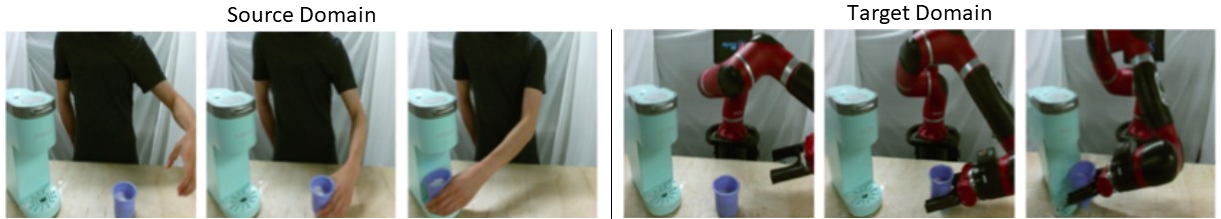
\includegraphics[width=0.9\textwidth]{Figures/images/embodiment_mismatch/embo.png}
    \caption{Representation of embodiment mismatch problem. (Left) The source domain represented by a video of human performing a task. (Right) The target domain, represented by the robot that executes the observed task.}
    \label{fig:embodiment}
\end{figure}

First of all, the points \textbf{(1)} and \textbf{(2)} are going to be answered. Regarding, the embodiment mismatch, this may happen, for example, when the video demonstration shows a human performing a task, but the goal is to train a robot (Figure \ref{fig:embodiment}).
To solve this problem, in \cite{smith2019avid,xiong2021learning_by_watching,li2021meta_watching_video_demonstration}, some sort of image-to-image translation was performed,  while in \cite{zakka2022xirl} the \textit{Temporal-Cycle Consistency} (TCC) \cite{dwibedi2019tcc} was used.
\newline In particular, in \cite{smith2019avid,li2021meta_watching_video_demonstration}, the Cycle-GAN \cite{zhu2017cycle_gan} was used to translate image from the source domain (human image) into the corresponding target domain (robot image). The need for an unsupervised image-to-image translation architecture such as the Cycle-GAN arises from the fact that there are not paired images. The network learns two mappings, the first from the source to the target domain $G : X \rightarrow Y$, the second from the target to the source domain $F : Y \rightarrow X$. The dataset for the source domain was composed of human demonstrations as well as a small amount of ``random” data, in which the human moves around the scene but does not specifically attempt the task, while for the target domain, it consists of  robot images executing randomly sampled actions in a few different settings. In \cite{xiong2021learning_by_watching} a similar approach was proposed, but the MUNIT \cite{huang2018munit} architecture was adopted for the image-to-image translation. With respect to the mentioned works, in \cite{zakka2022xirl} a completely different approach has been proposed. Indeed, starting from a set of video demonstrations characterized by both different length and demonstrator embodiment, the TCC approach was used to learn an encoder able to map demonstration frame into the corresponding embodiment-independent embedding. The idea behind TCC was to learn a correspondence between frames of different videos representing the same overall action (Figure \ref{fig:xirl}).
%To do so, for each video $S$ and $T$, of length $N$ and $M$, the frames embedding, $U$ and $V$, are computed. Then one embedding from $U$ is sampled, $u_{i} \in U$, and the nearest neighbor $\tilde{v} = \sum_{j}^M \alpha_{j}v_{j}$ is computed, where $\alpha$ is the result of a soft-max function, at the end the similarity vector $\boldsymbol{\beta}$ is computed between $\tilde{v}$ and each embedding in $U$ by means of a soft-max function. Since $\boldsymbol{\beta}$ is a distribution of probability, assumed to be Gaussian, the whole system is trained by imposing that the peak of $\boldsymbol{\beta}$ must appear at index $i$ (Figure \ref{}.
\begin{figure}[htb]
    \centering
    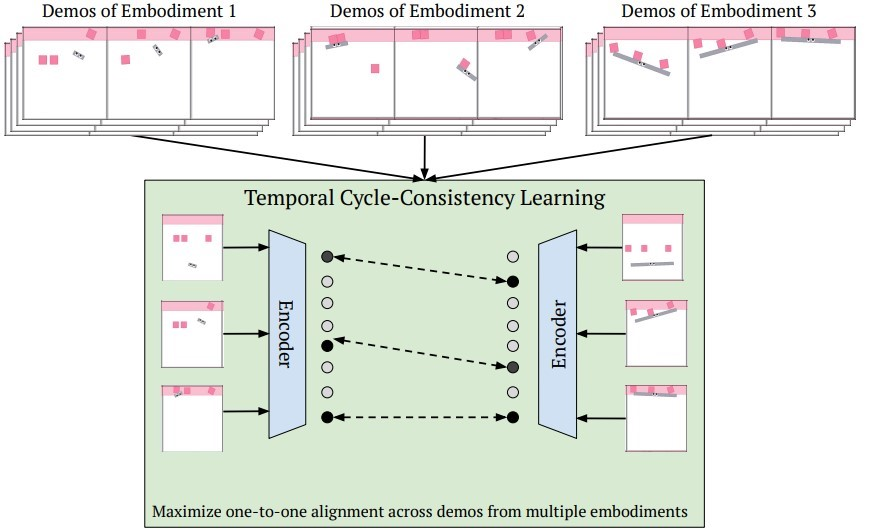
\includegraphics[width=0.65\textwidth]{Figures/images/xirl/xirl.jpg}
    \caption{Temporal-Cycle Consistency representation, used to learn an embodiment-agnostic encoder in \cite{zakka2022xirl}}
    \label{fig:xirl}
\end{figure}

\newline The correspondence problem between different viewpoints was faced by \cite{sermanet2018time_contrastive,liu2018imitation_from_observation}. In \cite{sermanet2018time_contrastive} a Convolutional Neural Network was trained by means of a \textit{Triplet-Loss} \cite{schroff2015triplet_loss}. The idea was to train a network able to predict an embedding independent from the view-point, but which contains only task relevant features. To reach this objective the network has to produce an embedding, $f(x)$, such that $|| f(x^{a}_{i}) - f(x^{p}_{i})||^{2}_{2} + \alpha < || f(x^{a}_{i}) - f(x^{n}_{i})||^{2}_{2}$ $\forall (f(x^{a}_{i}), f(x^{p}_{i}), f(x^{n}_{i})) \in \mathcal{T}$, where $\mathcal{T}$ is the set of all possible triplets in the dataset. This means that embedding produced by samples coming from different viewpoints, but that share the same time-step, $(x^{a}_{i},x^{p}_{i})$, should have a similar embedding, while embedding produced by samples coming from the same viewpoint, but in different time-step, $(x^{a}_{i},x^{n}_{i})$, should have a different embedding (Figure \ref{fig:time_contrastive}). In \cite{liu2018imitation_from_observation}, a different approach was used, indeed, a \textit{context translation problem} was solved by means of an Encoder-Decoder architecture (Figure \ref{fig:context-translation}). The proposed architecture was trained on pairs of demonstrations, $\mathcal{D}_{i}=[o^{i}_{0},o^{i}_{1},\dots,o^{i}_{T}]$ and $\mathcal{D}_{j}=[o^{j}_{0},o^{j}_{1},\dots,o^{j}_{T}]$ composed of visual observations. Samples in $D_{i}$ comes from the source context $\omega_{i}$, while samples in $\mathcal{D}_{j}$ comes from the target context $\omega_{j}$. The model must output the observations in $D_{j}$ conditioned on both $\mathcal{D}_{i}$ and the first observation $o^{j}_{0}$ from the target domain. As it will be explained next, the output of both the Time-Contrastive and the Context-Translation network can be used to obtain an engineered reward function.
\begin{figure}[htbp]
    \centering
    \begin{subfigure}[b]{0.45\textwidth}
        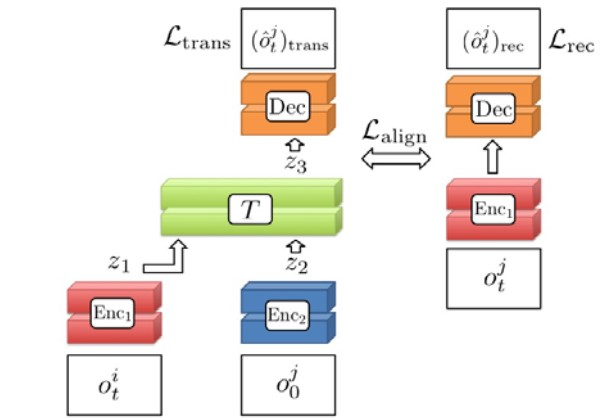
\includegraphics[width=\textwidth]{Figures/images/view_point_mismatch/context-translation-model.jpg}
        \caption{Context-Translation network, proposed in \cite{liu2018imitation_from_observation}}
        \label{fig:context-translation}
    \end{subfigure}
     \hfill
    \begin{subfigure}[b]{0.50\textwidth}
        \centering
        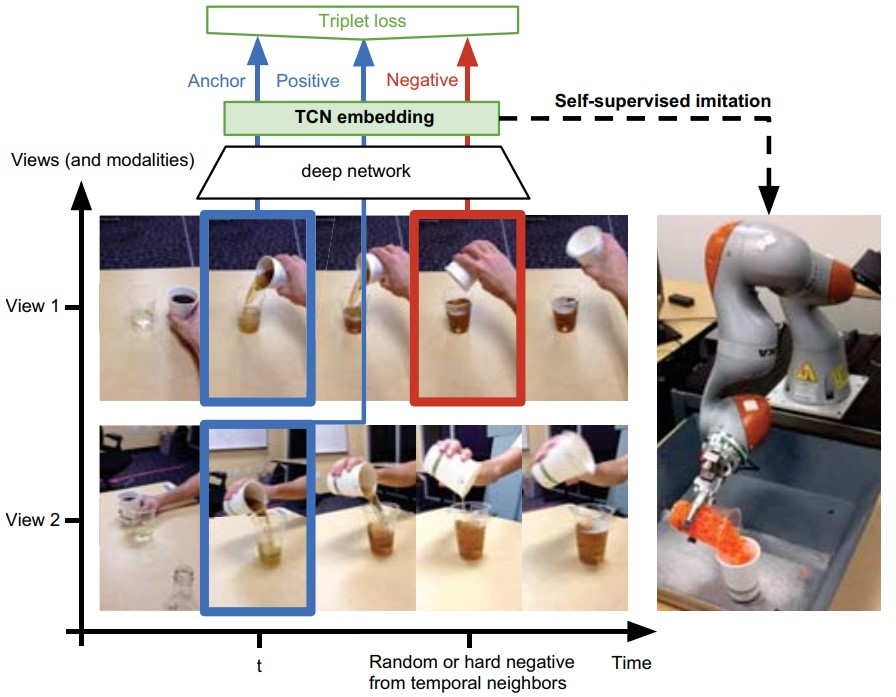
\includegraphics[width=\textwidth]{Figures/images/view_point_mismatch/time-contrastive-network.jpg}
        \caption{Time-Contrastive network, proposed in \cite{sermanet2018time_contrastive}.}
        \label{fig:time_contrastive}
    \end{subfigure}
    \caption{Examples of how the mismatch between demonstrator viewpoint and learner viewpoint can be handled.}
    \label{fig:differet_viewpoint}
\end{figure}


Concerning the way how the policy can be obtained, it is necessary to distinguish between Model-Based and Model-Free methods.
\newline Among \textbf{Model-Free} methods, a further classification must be made between methods based on \textit{Reward Engineering} and \textit{Adversarial Learning}.
\newline Methods based on Reward Engineering are \cite{liu2018imitation_from_observation,sermanet2018time_contrastive,xiong2021learning_by_watching,zakka2022xirl}, in which a hand-designed reward function is used to train a RL agent. In particular, the reward functions obtained in the cited works leverage some sort of \textit{Feature Tracking}. In \cite{liu2018imitation_from_observation} the reward function was $R(o^{l}_{t}) = -||Enc_{1}(o^{l}_{t}) - \frac{1}{n} \sum_{i}^{n}F(o_{t}^{i},o_{0}^{l})||^{2}_{2} - w_{rec} (||o^{l}_{t} - \frac{1}{n} \sum_{i}^{n}M(o_{t}^{i},o_{0}^{l})||^{2}_{2})$. The first term is the classic Feature Tracking reward function, where the goal is to minimize the Euclidian Distance between the encoding of the current learner observation $o^{l}_{t}$ and the encoding of the demonstration in the learner context, the second term has the aim to penalize the policy for experiencing observations that differ from the translated observation.
In \cite{sermanet2018time_contrastive}, the reward function was $R(\textbf{v}_{t}, \textbf{w}_{t}) = - \alpha || \ \textbf{w}_{t} - \textbf{v}_{t} \ ||^{2}_{2} - \beta \sqrt{\gamma + || \ \textbf{w}_{t} - \textbf{v}_{t} \ ||^{2}_{2}}$, where $\textbf{v}_{t}$ is the TCN embedding of the video demonstration at timestep t, while $\textbf{w}_{t}$ is the TCN embedding produced by the robot observation (Figure \ref{fig:time_contrastive}).
In \cite{xiong2021learning_by_watching}, a keypoint-representation is obtained for both current robot observations $z_{t}$, and for each frames of the translated demonstration video $\left\{z^{E}_{p}\right\}_{p=1}^{T}$. Then, the reward is computed as $R(z_{t},z_{t+1},z^{E}) = - \lambda_{1} \underset{p}{min} ||z_{t}-z^{E}_{p}|| - \lambda_{2} \underset{p}{min} ||(z_{t+1}-z_{t}) - (z^{E}_{p+1}-z^{E}_{p})||$. %(Figure \ref{fig:lbw}). 
In \cite{zakka2022xirl}, the reward function was defined as $R(s_{t}) = -\frac{1}{k} \ || \phi(s_{t}) - g||^{2}_{2}$, where $g$ is the goal embedding, defined as the mean embedding of the last frame of all the demonstration videos in the dataset, while $\phi(s_{t})$ is the embedding of the current observation. Experimental results, on simulation data proved that the proposed method can be used to learn tasks from cross-embodiment demonstrations, outperforming baseline \cite{sermanet2018time_contrastive} in terms of both sample efficiency and performance.%\begin{figure}[htb]
    \centering
    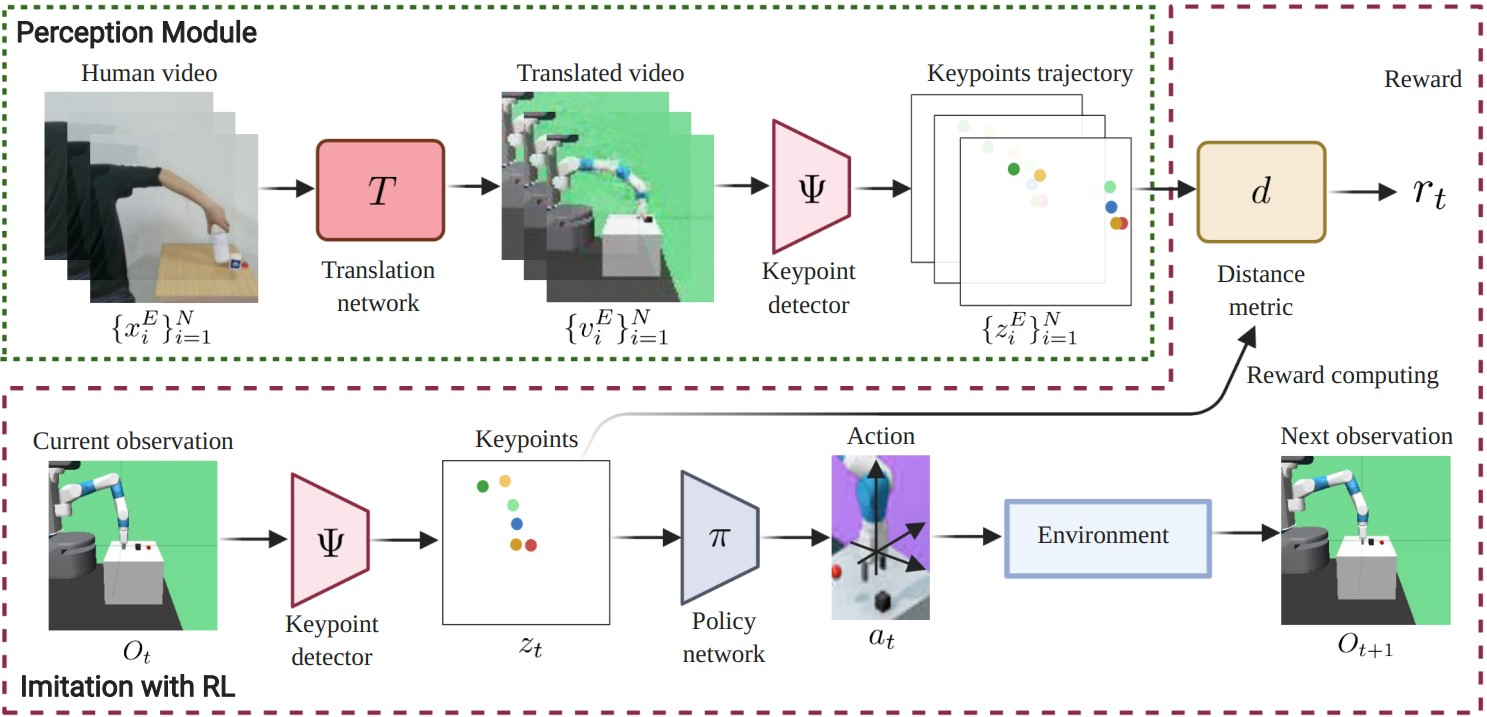
\includegraphics[width=0.7\textwidth]{Figures/images/learning_by_watching/learning_by_watching.jpg}
    \caption{Architecture proposed by \cite{xiong2021learning_by_watching}}
    \label{fig:lbw}
\end{figure}

\newline Regarding the methods based on Adversarial Learning, there are \cite{merel2017learning,torabi2018gaifo}. Obviously, these methods are strictly related to the Generative Adversarial Imitation Learning setting. However, with respect to the methods presented in GAIL paragraph (pag. \pageref{para:gail}), these methods do not assume access to the demonstrator action. Indeed, the goal of the preliminary work \cite{merel2017learning} was to prove that the Adversarial Learning Setting can be effectively used even without the action information. To prove this hypothesis, the authors performed a series of experiments in simulation for a walking task, where the same RL policy was trained in two contexts, the first, where the Discriminator had access to the (state, action) pair, the second where the Discriminator had access to state only demonstrations. The results obtained did not show a substantial difference between the two settings, supporting the hypothesis that in task learning the essential information is contained in the state.
\begin{algorithm}
\caption{GAIfO algorithm \cite{torabi2018gaifo}}
\label{alg:gaifo_algorithm}
\begin{algorithmic}
\Require Initial policy $\pi^{L}_{\phi}$, Initial Discriminator $D_{\theta}$
\Require State-only expert demonstration trajectories $\tau^{E} = \left \{ (s,s') \right \}$
\While {Policy Improves}
    \State Execute $\pi^{L}_{\phi}$ and collect state transitions $\tau^{L} = \left \{ (s,s') \right \}$
    \State Update $D_{\theta}$, with $\mathcal{L}_{D_{\theta}} = - \ ( \ \mathbb{E}_{\tau^{L}}[\log (D_{\theta}(s, s')) ] + \mathbb{E}_{\tau^{E}}[\log(1 - D_{\theta}(s, s'))] \ )$
    \State Update $\pi^{L}_{\phi}$, with reward $ r_{\pi^{L}_{\phi}} = - \ ( \ \mathbb{E}_{\tau^{L}}[\log(D_{\theta}(s, s'))] \ )$
\EndWhile
\end{algorithmic}
\end{algorithm}
\newline The next remarkable work was proposed by the authors of \cite{torabi2018gaifo}, that formalized the \textit{GAIfO} algorithm, (Algorithm \ref{alg:gaifo_algorithm}), that is an extension to state-only demonstration of GAIL \cite{ho2016gail}. The proposed algorithm was used to train a network to solve tasks in simulation environment \cite{brockman2016openai}, with both low-dimensional state representation, and visual-state representation. Results with respect to the number of demonstrated trajectories are reported in Figure \ref{fig:gaifo_results}.
As it can be noted from the results, GAIfO outperforms previous observation based methods \cite{sermanet2018time_contrastive,torabi2018bco}, in a setting with a low number of expert trajectories. The main drawback of GAIfO is the high number of environmental interactions needed to learn a policy, since the model-free TRPO \cite{schulman2015trpo} algorithm was used to train the policy. This problem was solved by DEALIO \cite{torabi2021dealio}, which replaced the model-free algorithm with PILQR \cite{chebotar2017pilqr} the model-based RL algorithm reported next. \begin{figure}[htbp]
     \centering
     \begin{subfigure}[b]{0.8\textwidth}
        \centering
         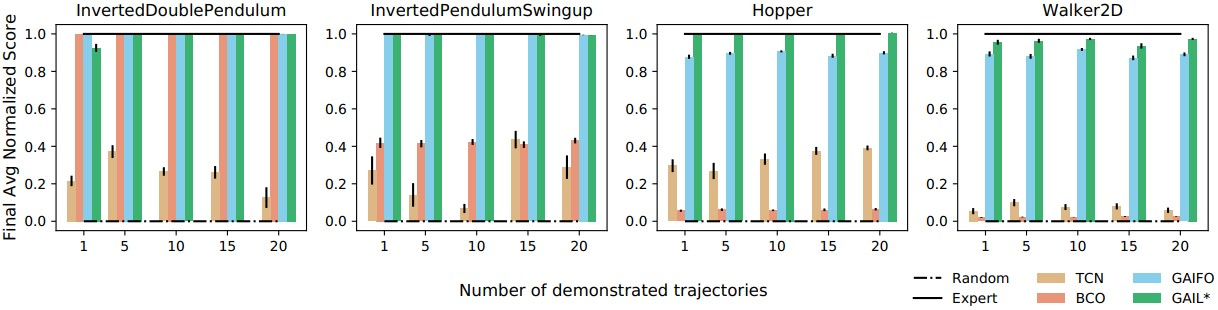
\includegraphics[width=\textwidth]{Figures/images/gaifo_results/gaifo_results.jpg}
         \caption{Experimental results in low-dimensional state space}
         \label{fig:low_dimensional}
     \end{subfigure}

     \begin{subfigure}[b]{0.8\textwidth}
        \centering
         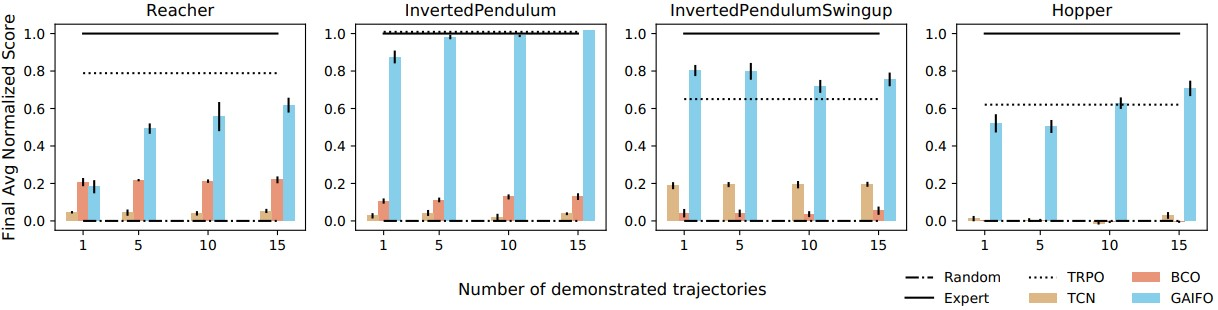
\includegraphics[width=\textwidth]{Figures/images/gaifo_results/gaifo_results_visual.jpg}
         \caption{Experimental results in high-dimensional state space}
         \label{fig:high_dimensional}
     \end{subfigure}
    \hfill
    \caption{Experimental results reported in \cite{torabi2018gaifo}.}
    \label{fig:gaifo_results}
\end{figure}


%result of the Proposition \ref{}, that is an extension to state-only of the Proposition \ref{}, combined with the generative adversarial regularizer in Formula \ref{} characterized by the conjugate in Formula \ref{} 
%\begin{prop}
\label{pre:gaifo_preposition}
$RL\circ  IRLfO_{\psi}$ and $ arg \ min_{\pi^{L} \ \in \ \Pi} \ \psi^{*}(\rho^{s}_{\pi^{L}} - \rho^{s}_{\pi^{E}})$ induce policies that have the same state-transition occupancy measure, $\rho^{s}_{\tilde{\pi}}$
\end{prop}. 
\noindent Among the \textbf{Model-Based} methods a further classification has to be made between methods that obtain the \textit{Inverse Dynamic Model} and methods that obtain the \textit{Forward Dynamic Model}. The former, given in input a transition $(s_{t}, s_{t+1})$, obtain a function $M$, able to map state transition to action i.e., $a_{t} = M(s_{t}, s_{t+1})$. While the latter, given in input a state-action pair $(s_{t}, a_{t})$, aim to learn a function $F$ able to generate the next state $s_{t+1}$, i.e., $s_{t+1} = T(s_{t}, a_{t})$.
\newline Methods that obtain  the Inverse Dynamic Model are \cite{nair2017combining,torabi2018bco,guo2019hybrid_rl,radosavovic2021state_only_demo}. In \cite{nair2017combining} the goal was to obtain a system capable of tying the knot to a rope. To achieve it, a self-supervised learning approach was used to train a Convolutional Neural Network, that, taken in input a pair of images $(I_{t}, I_{t+1})$ representing two successive rope states, was able to obtain the action to perform in order to reach the state $I_{t+1}$ from $I_{t}$. To train the proposed network, a dataset composed of 30K tuples $(I_{t},a_{t},I_{t+1})$ was collected by means of an exploratory policy. Authors in \cite{torabi2018bco} proposed a general approach, depicted in Figure \ref{fig:bco}, and composed by two main parts, the learned Inverse Dynamic Model, $M_{\theta}$, and the learned policy $\pi_{\phi}$. In its general form, the learning procedure is an iterative procedure, where the model $M_{\theta}^{i}$ is updated by maximizing the probability $p_{\theta}(a_{t}|s_{t},s_{t+1})$, where the tuples $(s_{t},a_{t},s_{t+1})$ are collected by running the current policy. Once the dynamic model is updated then it is used to infer the action $\tilde{a}_{t}$ given the demonstrations. At the end, since the policy has access to both state and action information, classic BC learning can be run, optimizing the policy parameters through maximum-likelihood estimation $\phi^{*} = \underset{\phi}{argmax} \prod_{i=0}^{N} \pi^{L}_{\phi}(\tilde{a}_{i}|s_{i})$. In \cite{guo2019hybrid_rl}, the same approach as in \cite{torabi2018bco}, but the agent's policy was trained according to a linear combination of Behavioral Cloning and Advantage Actor Critic (A2C) objective function \cite{mnih2016a2c}, i.e., $\mathcal{L}^{hyb}_{\theta} = \mathbb{E}_{s,a}[A(s)\log(a|s;\theta)+\alpha \ \mathcal{H}(\pi^{L}(.|s))] + \mathbb{E}_{(\hat{s}_{t},\hat{s}_{t+1})\sim D}[\log(\pi^{L}(M(\hat{s}_{t},\hat{s}_{t+1})|\theta)]$. Here, the main problem is the assumption to have access to reward function, which can reduce its applicability in real-robot manipulation tasks. In \cite{radosavovic2021state_only_demo}, the work in \cite{Rajeswaran18_learning_complex_dexterous} was extended to state-only demonstration, and the \textit{State-Only Imitation Learning} (SOIL) algorithm was proposed. The context is the one of complex dexterous manipulation, i.e., a simulated humanoid hand must be able to perform tasks such as object reallocation, tool use, in-hand manipulation, and door opening. A neural network was trained to represent the Inverse Dynamic Model, by minimizing the L2-loss, given in input the action performed during the policy rollout. Then, the policy was updated according to \textit{Demo Augmented Policy Gradient} (DAPG) \cite{Rajeswaran18_learning_complex_dexterous}, adapted for state-only demonstration, i.e., $g_{SOIL} = g + \lambda_{0} \ \lambda_{1}^{k} \ \sum_{(s_{t},\tilde{a}_{t} \in D')} \nabla_{\theta}\log\pi^{L}_{\theta}(\tilde{a}_{t},s_{t})$, where $g$ is the Natural Policy Gradient term. The idea is to leverage the demonstrations at the beginning of the training, then exploit the RL algorithm to improve the behavior itself. Indeed, experiments performed in simulation, proved that, with respect to pure RL, the proposed method converges faster, and producing more human-like behaviors.
\begin{figure}[htb]
    \centering
    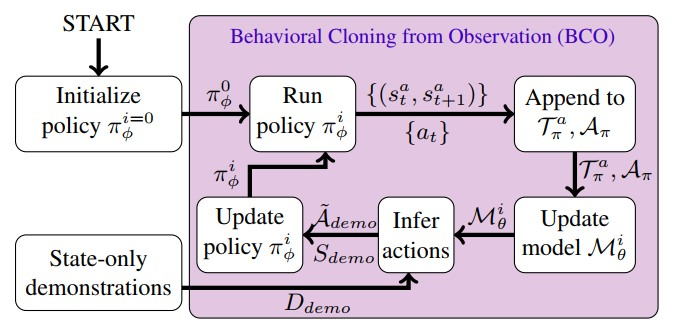
\includegraphics[width=0.6\textwidth]{Figures/images/bco/bco.jpg}
    \caption{Representation of the learning procedure proposed by \cite{torabi2018bco}}
    \label{fig:bco}
\end{figure}

\newline Methods that obtain the Forward Dynamic Model are \cite{smith2019avid,torabi2021dealio}. In \cite{smith2019avid}, once the human video demonstration has been translated into the corresponding robot video, the policy was learned according to the model-based RL algorithm SOLARIS \cite{zhang2019solar}, which allows to obtain a controller optimized according to Linear-Quadratic Regulator (LQR) procedure. The idea was to optimize the policy in a low-dimensional high-regularized \textit{latent space}, generated according to Variational Inference \cite{Kingma2014_vae}. Starting from a sequence of observation-action, a Global Dynamic Model over latent trajectory is obtained. Then, given the Latent Dynamic Model, a Linear-Gaussian Controller is obtained through LQR-FLM \cite{levine2014lqr_flm}. Real world robotic experiments, shown that with \textbf{2 hours} of robot interaction it was possible to outperform previous works such as \cite{sermanet2018time_contrastive,torabi2018bco} and classic BC algorithm, on tasks such as ``coffee making" (Figure \ref{fig:embodiment}) and cup-retrieving (i.e., the robot has to take a cup from a closed drawer).
In \cite{torabi2021dealio} the sample-inefficiency problem of GAIfO \cite{torabi2018gaifo} was addressed. The idea was to exploit the adversarial learning setting with state-only demonstration, which has shown promising results (Figure \ref{fig:gaifo_results}), and combining it with a more data-efficient RL algorithm, such as PILQR \cite{chebotar2017pilqr}. The core of PILQR is the LQR optimization procedure. Generally speaking, it returns a \textit{linear-gaussian controller} (Formula \ref{formula:linear_gaussian_controller}), that optimizes a \textit{quadratic-cost function} (Formula \ref{formula:quadratic_cost_function}), under the assumption of \textit{linear-gaussian dynamic} (Formula \ref{formula:gaussian_dyn}).\begin{equation}
\label{formula:linear_gaussian_controller}
    \pi(a_{t}|s_{t}) = \mathcal{N}(K_{t}s_{t} + k_{t}, S_{t})
\end{equation}

\begin{equation}
\label{formula:quadratic_cost_function}
c(s_{t},a_{t}) = \begin{bmatrix}
s_{t}
\\ 
a_{t}
\end{bmatrix}^{T}C_{t}\begin{bmatrix}
s_{t}
\\ 
a_{t}
\end{bmatrix} + \begin{bmatrix}
s_{t}
\\ 
a_{t}
\end{bmatrix}^{T} c_{t} + cc_{t}
\end{equation}

\begin{equation}
\label{formula:gaussian_dyn}
s_{t+1} \sim P(s_{t+1}|s_{t},a_{t}) = \mathcal{N}(F_{t}
\begin{bmatrix}
s_{t}
\\ 
a_{t}
\end{bmatrix} + f_{t}, \Sigma_{t})
\end{equation}


\noindent In order to use this framework, the linear-gaussian dynamic model was fitted starting from the current policy rollouts, then, to obtain a quadratic cost function as needed by LQR, the dynamic model was used to express the modified discriminator output (Formula \ref{formula:output_discriminator}) as function of the pair $(s_{t},a_{t})$.
\begin{equation}
\label{formula:output_discriminator}
D_{\theta}(s_{t},s_{t+1}) = \frac{1}{2}
\begin{bmatrix}
s_{t}
\\ 
s_{t+1}
\end{bmatrix}^{T}C^{ss}(s_{t},s_{t+1})
\begin{bmatrix}
s_{t}
\\ 
s_{t+1}
\end{bmatrix} + \begin{bmatrix}
s_{t}
\\ 
s_{t+1}
\end{bmatrix}^{T} c^{ss}(s_{t}, s_{t+1})
\end{equation}
Experiments performed in simulation with low-dimensional state space have shown promising results (Figure \ref{fig:dealio_performance}), in terms of sample-efficiency with respect to the GAIfO baseline. However, improvements would be made in order to: \begin{enumerate*}[label=\textbf{(\arabic*)}]
    \item reduce the variance, in order to make the learning process more reliable,
    \item increase the overall performance,
    \item adapt the algorithm to work with real-world robot manipulation tasks.
\end{enumerate*}
\begin{figure}[htbp]
    \centering
    \begin{subfigure}[b]{0.76\textwidth}
        \centering
        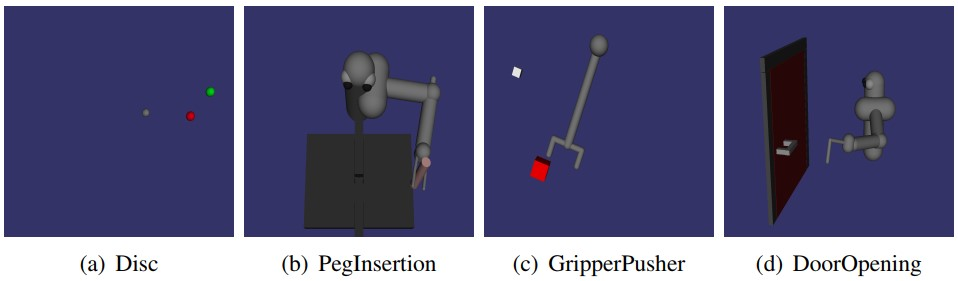
\includegraphics[width=\textwidth]{Figures/images/dealio/dealio_performed_task.jpg}
        \caption{Control Tasks solved in \cite{torabi2021dealio}}
        \label{fig:dealio_task}
    \end{subfigure}
    \hfill
    
    \begin{subfigure}[b]{0.9\textwidth}
        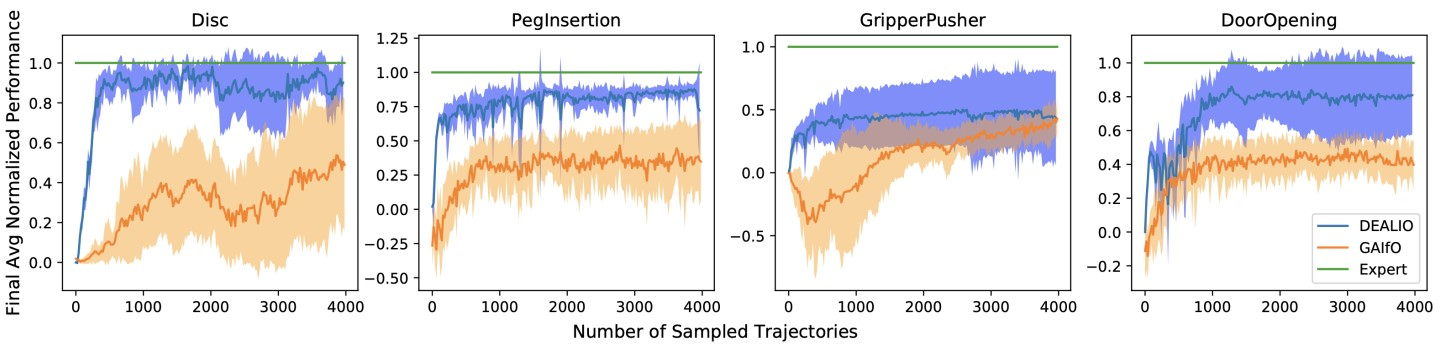
\includegraphics[width=\textwidth]{Figures/images/dealio/dealio_performance.jpg}
        \caption{Performance of DEALIO \cite{torabi2021dealio} compared against GAIfO \cite{torabi2018gaifo}, with respect to the number of trajectories sampled during the learning process.}
        \label{fig:dealio_performance}
    \end{subfigure}
    \caption{DEAILO: (\ref{fig:dealio_task}) Control Tasks, (\ref{fig:dealio_performance}) Performance Level}
    \label{fig:dealio}
\end{figure}


Generally, LfO methods have demonstrated interesting features, such as generating a policy from state-based information alone, supporting the hypothesis that the primary source of information for task learning is the sequence of state transitions. Extrapolating the valuable information to perform actions that induce the desired behavior may not be trivial, mainly if the state space is represented by images of a human operator, leading to the design of architectures composed of different stages, which increase not only the complexity of the system itself but also the amount and diversity of data required for their training. In addition, many methods of interest have been tested in simulated or otherwise relatively simple scenarios, still leaving open the question of whether these methods can be used in real-world complex robotic manipulation tasks.